In the previous Chapter, we explored the time evolution of a wave function governed by the evolution operator, $\hat{U}(t)$, and introduced a simple numerical technique for propagating the wave function. This way we can study dynamical processes governed by quantum mechanics and explore intricacies of the quantum world like interference or tunnelling. However, the time evolution of a wave function offers more than just insight into the system's dynamics -- it also encodes the energy spectrum of the system. Although counter-intuitive, we can obtain the energy spectrum, a time-independent quantity usually calculated by solving the \acrfull{tise}, by performing a dynamical simulation. This time-dependent perspective is widely used in theoretical spectroscopy where both the energy spectrum and intensities are calculated from quantum or semiclassical dynamics.

\section{Theoretical background}
\label{sec:autocorrintro}

To understand how the energy spectrum is encoded in the wave function propagation, we examine the exact solution of the \acrlong{tdse}. Assume we could solve the \acrshort{tise}
\begin{equation}
    \hat{H}(x) \phi_k(x) = E_k \phi_k(x)
    \label{eq:tise0}
\end{equation}
and obtain a complete set of eigenfunctions $\phi_k(x)$.\footnote{In practice, obtaining these eigenfunctions is often the most challenging step in this approach, as they cannot usually be computed directly. Therefore, this method is more useful for deriving theoretical insights rather than for practical calculations.} This set of eignefunctions forms an orthonormal basis, allowing us to expand any wave function as a linear combination of $\phi_k$. Expanding the initial wave function in this basis, we write:
\begin{equation}
    \psi(x,0) = \sum_k c_k \phi_k(x) \, ,
\end{equation}
where $c_k$ are the expansion coefficients determined as 
\begin{equation}
    c_k = \langle \phi_k(x) | \psi(x,0) \rangle = \int_{-\infty}^\infty \phi_k^*(x) \psi(x,0) \dd x \, .
    \label{eq:psi0v1}
\end{equation}
If the initial wave function is normalized, the expansion coefficients further fulfil the following condition
\begin{equation}
    \sum_k |c_k|^2 = 1 \, .
    \label{eq:initcoeffs}
\end{equation}

The solution of the \acrshort{tdse}, $\psi(x,t)$, can be calculated by applying the propagator $\hat{U}(t)$ to the initial wave function (Eqs.~\eqref{eq:U} and~\eqref{eq:U1}):
\begin{equation}
    \psi(x,t) = \hat{U}(t)\psi(x,0) = \e^{-\frac{i}{\hbar}\hat{H}(x)t} \psi(x,0) = \sum_k c_k \e^{-\frac{i}{\hbar}\hat{H}(x)t} \phi_k(x) \, .
\end{equation}
Since $\phi_k$ are eigenfunctions of the Hamiltonian $\hat{H}$, the propagator acts on each $\phi_k$ as:
\begin{equation}
    \e^{-\frac{i}{\hbar}\hat{H}(x)t} \phi_k(x) = \e^{-\frac{i}{\hbar}E_k t} \phi_k(x) \, ,
\end{equation}
leading to the time-dependent solution:
\begin{equation}
    \psi(x,t) = \sum_k c_k \e^{-\frac{i}{\hbar}E_k t}\phi_k(x) \, .
    \label{eq:tdpsi1}
\end{equation}
This expression represents the exact solution of the \acrshort{tdse} in the basis of Hamiltonian eigenstates. For time-independent Hamiltonians (i.e., $\hat{H} \neq \hat{H}(t)$), the coefficients $c_k$ remain constant over time, and the only time-dependent terms are the exponentials $\e^{-\frac{i}{\hbar}E_k t}$, fully governing the evolution.

Using this exact \acrshort{tdse} solution, we can now extract the energy spectrum through the \textit{autocorrelation function}. The autocorrelation function is defined as an overlap of the wave function at time $t$ with the initial wave function at time 0:
\begin{equation}
    S(t) = \langle \psi(x,0) | \psi(x,t) \rangle =\int_{-\infty}^{\infty}\psi^*(x,0) \psi(x,t) \dd x\, .
\end{equation}
It measures the probability amplitude of $\psi(x,t)$ being in the initial state $\psi(x,0)$. Thus, the autocorrelation function is always equal to 1 at time 0. Inserting the exact solution of \acrshort{tdse} \eqref{eq:tdpsi1}, the autocorrelation function reads
\begin{align}
    S(t) &= \int_{-\infty}^{\infty} \sum_l \sum_k c_l^* \phi_l^*(x) c_k \e^{-\frac{i}{\hbar}E_k t}\phi_k(x) \dd x \notag\\
    &= \sum_l \sum_k c^*_l c_k \e^{-\frac{i}{\hbar}E_k t} \int_{-\infty}^{\infty}  \phi_l^*(x) \phi_k(x) \dd x \notag\\
    &= \sum_l \sum_k c^*_l c_k \e^{-\frac{i}{\hbar}E_k t} \delta_{kl} \notag\\
    &= \sum_k |c_k|^2 \e^{-\frac{i}{\hbar}E_k t} \, .
\end{align}
It appears that the autocorrelation function is a sum of the time-dependent exponentials weighted by magnitudes of the coefficients $c_k$. The energy spectrum $\sigma$ can then be obtained by applying \acrshort{ift} to the autocorrelation function:
\begin{equation}
    \sigma(E) = \int_{-\infty}^{\infty} S(t) \e^{\frac{i}{\hbar}Et} \dd t  = \sum_k |c_k|^2 \int_{-\infty}^{\infty} \e^{\frac{i}{\hbar}(E-E_k)t} \dd t = \sum_k |c_k|^2 \delta(E-E_k) \, ,
    \label{eq:autocorr1}
\end{equation}
where the Dirac $\delta$-distributions are centred at energies $E_k$ with magnitudes $|c_k|^2$. Thus, the spectrum exhibits peaks at all eigenvalues $E_k$ for which $c_k\neq 0$ in the initial wave function $\psi(x,0)$, see Fig.~\ref{eq:autocorr1}.

\begin{figure}[ht!]
    \centering
    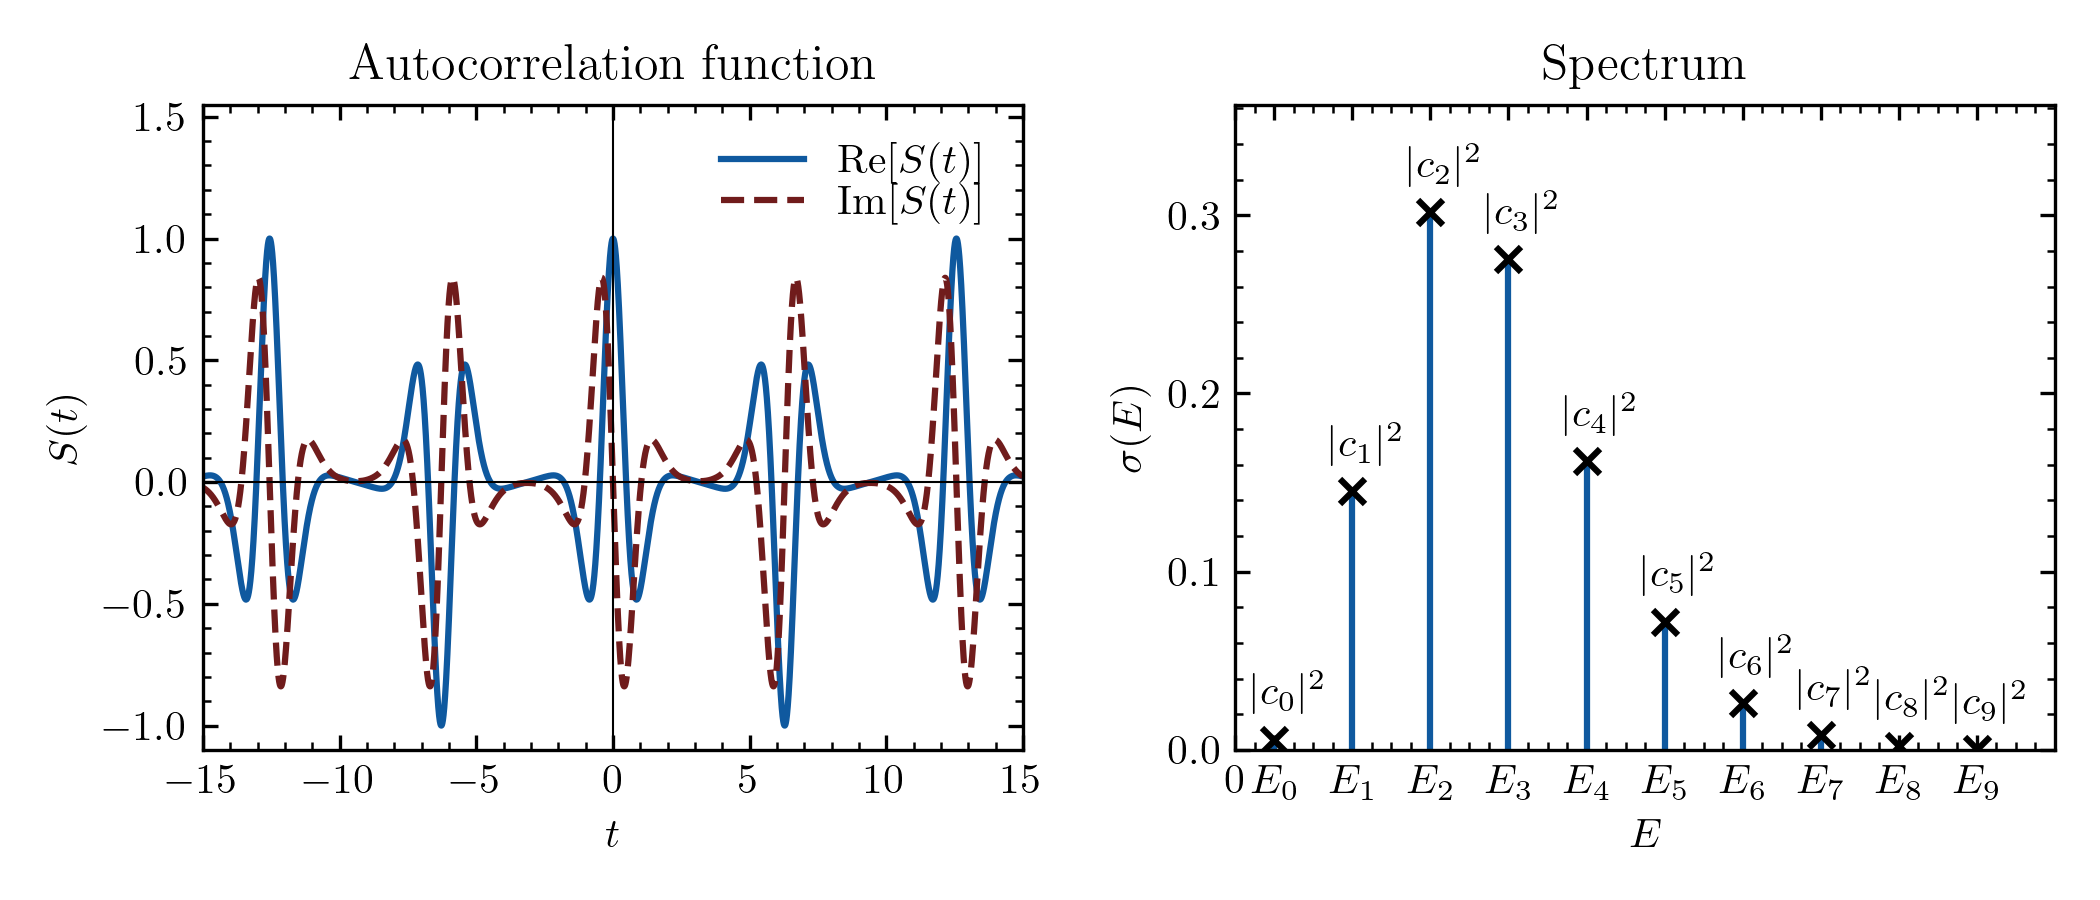
\includegraphics[width=0.9\linewidth]{scriptum/obrazky/autocorr/autocorr1.png}
    \caption{An illustrative example of autocorrelation function $S(t)$ of a harmonic oscillator (left) and its corresponding energy spectrum $\sigma(E)$ (right).}
    \label{fig:autocorr1}
\end{figure}

Although this analysis is based on the exact TDSE solution and the full set of eigenfunctions $\phi_k$, the derived autocorrelation function $S(t)$ and energy spectrum $\sigma(E)$ apply to any wave function evolution. This method provides a powerful tool for calculating the spectrum of any Hamiltonian by time-propagating a wave function, which is often computationally more feasible than directly diagonalizing the Hamiltonian.


\section{Numerical implementation}
\label{sec:autocorr_numap}

The numerical implementation of the outlined procedure for calculating the energy spectrum from the autocorrelation function is straightforward. We need to perform a quantum dynamical simulation as described in Chapter~\ref{kap:qd} and calculate the overlap between $\psi(x,t)$ and $\psi(x,0)$ at each step. The overlaps form the autocorrelation function $S(t)$ which is then converted into the energy spectrum by the \acrlong{ift} after the simulation. However, the integral in the \acrlong{ift} in Eq.~\eqref{eq:autocorr1} runs from time $-\infty$ to $\infty$ requiring the knowledge of the autocorrelation function from $-\infty$ to $\infty$, which is usually unavailable since a typical simulation runs only from time 0 to some finite time $t_\mathrm{max}$. Thus, we have only truncated information about $S(t)$ in the positive times and lack the information about negative times.

The lack of information about $S(t)$ in negative times can be addressed by exploring the properties of the autocorrelation function.
\begin{align}
    S^*(t) &= \langle \psi(x,0) | \psi(x,t) \rangle^* = \langle \psi(x,0) | \e^{-\frac{i}{\hbar}\hat{H}(x)t} |\psi(x,0) \rangle^* = \langle \psi(x,0) | \e^{\frac{i}{\hbar}\hat{H}(x)t} |\psi(x,0) \rangle \notag \\
    &= \langle \psi(x,0) | \e^{-\frac{i}{\hbar}\hat{H}(x)(-t)} |\psi(x,0) \rangle = S(-t) \, ,
    \label{eq:autocorrsym2}
\end{align}
where we have complex conjugated $S(t)$ and noticed we can compensate for the complex conjugation by taking the time negative. This leads to a fundamental symmetry of the autocorrelation function,
\begin{align}
    S(-t) = S^*(t) \, ,
    \label{eq:autocorrsym1}
\end{align}
which allows us to obtain the autocorrelation in negative times by taking it complex conjugate in the positive times. The symmetry of the autocorrelation function in Eq.~\eqref{eq:autocorrsym1} resolves our problems with the lack of information about negative times and saves us from propagating the wave function also back in time.

Although resolving the negative-time issue, we still have a problem with the truncated autocorrelation function at some time $t_\mathrm{max}$ due to a finite propagation of the wave function. Ideally, we want the autocorrelation function to decay to zero at $t_\mathrm{max}$. Then, the integral in Eq.~\eqref{eq:autocorrsym1} beyond $t_\mathrm{max}$ is zero and we can formally integrate only in limits $[-t_\mathrm{max}, t_\mathrm{max}]$. Thus, we always want to propagate the wave function until the autocorrelation function decays to zero. A decay of the autocorrelation function is common in natural processes such as photochemistry, luminescence or Auger decay. 

Nonetheless, the autocorrelation function does not decay naturally with time in systems we learned to simulate in Chapter~\ref{kap:qd}, since such decay would require coupling to some external bath or a multistate system. The autocorrelation function is then periodic and extends to infinity. In such cases, we need to attenuate the autocorrelation function artificially in order to decay within a feasible simulation time. This attenuation can be achieved by introducing a damping function $\xi$ which attenuates the autocorrelation function such that:
\begin{equation}
    \sigma(E) = \int_{-\infty}^{\infty} \xi(t) S(t) \e^{\frac{i}{\hbar}(E)t}  \dd t =  \int_{-t_\mathrm{max}}^{t_\mathrm{max}} \xi(t) S(t) \e^{\frac{i}{\hbar}(E)t}\, .
    \label{eq:damping1}
\end{equation}
Typical damping functions are an exponential, 
\begin{equation}
    \xi(t) = \e^{-\gamma t} \, ,
\end{equation}
or a  Gaussian function,
\begin{equation}
    \xi(t) = \e^{-\gamma t^2} \, .
    \label{eq:gaussdamping}
\end{equation}
The damping parameter $\gamma$ governs the strength of the attenuation. The damping has a profound effect on the spectra. Without the damping, the spectrum would be a sum of Dirac $\delta$-distributions, infinitely narrow peaks, with intensity corresponding to $|c_k|^2$, as seen in Figure~\ref{fig:autocorr1}. However, the damping introduces broadening of the peaks proportional to the damping factor $\gamma$. Thus, applying the damping function artificially broadens our peaks and limits our resolution of energy levels in the system as illustrated in Figure~\ref{fig:autocorr2}. It is always crucial to set the damping such that the broadening is smaller than the spacing between the eigenenergies.

\begin{figure}[ht!]
    \centering
    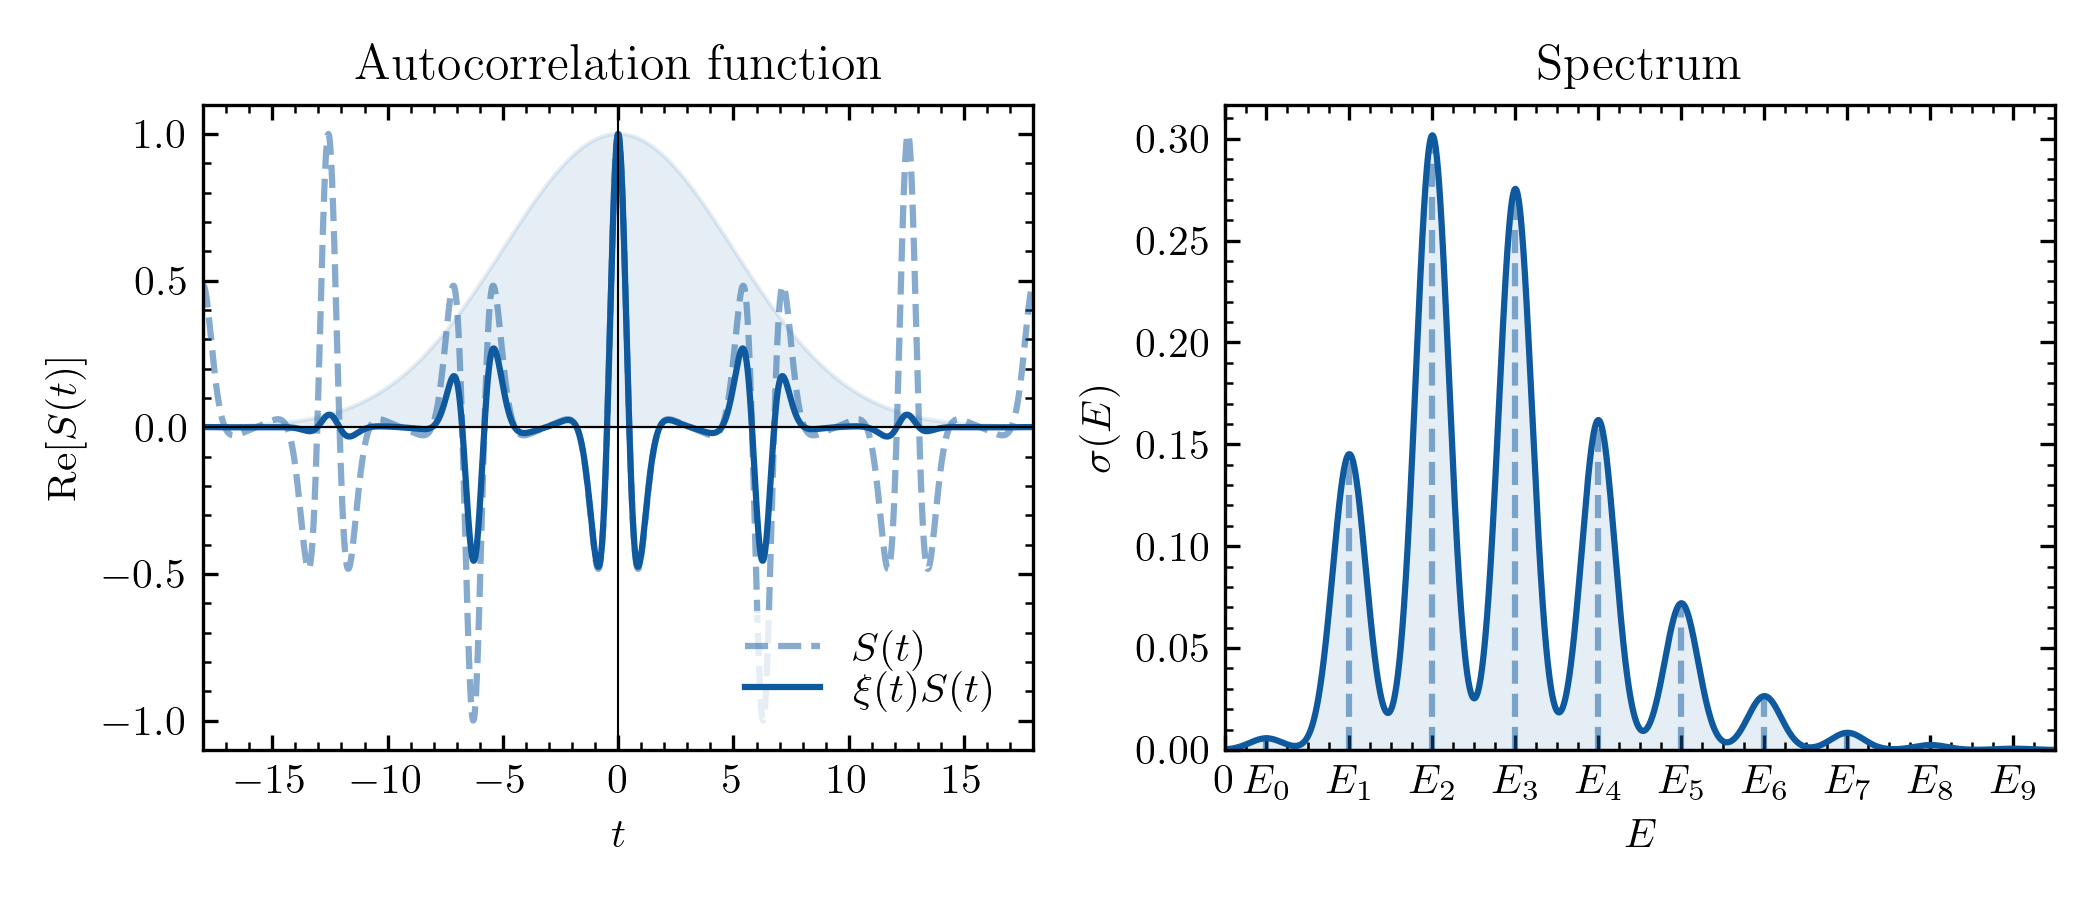
\includegraphics[width=0.9\linewidth]{scriptum/obrazky/autocorr/autocorr2.png}
    \caption{The effect of the damping function $\xi(t)$ on the energy spectrum calculated from the autocorrelation function. The damping of the autocorrelation function causes a broadening of the spectral lines but preserves the peak positions. If the damping is caused by a natural effect (fluorescence, internal conversion, Auger decay, etc.), the width of the spectral lines bears information about the lifetime of the damping process. For a very fast damping, the peaks can merge into one blurred spectrum without the possibility to distinguish the energy levels.}
    \label{fig:autocorr2}
\end{figure}

This completes our discussion on how to deal with a finite autocorrelation function spanning only the positive-time region. Let us now briefly comment on what would happen if we did not extend the autocorrelation function to negative times and attenuated it. The algorithms for discrete \acrshort{ift} would not prevent us from transforming an autocorrelation function spanning a range between 0 and $t_\mathrm{max}$. We would still get a spectrum in the energy domain, yet the spectrum would be plagued with some artefacts. Without deriving it, we just state that in the discrete \acrshort{ft} (or \acrshort{ift}), the signal obtained in the region of $[0, t_\mathrm{max}]$ is copied to $[t_\mathrm{max}, 2t_\mathrm{max}]$ and $[-t_\mathrm{max}, 0]$ and so on. This, first of all, breaks the symmetry of the autocorrelation function derived in Eq.~\eqref{eq:autocorrsym2} and, secondly, creates discontinuities in $S(t)$. The former causes an incorrect shape of the peaks in the spectrum while the latter causes so-called \textit{ringing} in the spectrum. Both effects decrease the resolution of the spectrum for smaller peaks and may lead to incorrect extraction of eigenenergies from the spectrum. The effect of damping and extending the autocorrelation function is explored in more detail in Figure~\ref{fig:autocorr3}.

\begin{figure}[ht!]
    \centering
    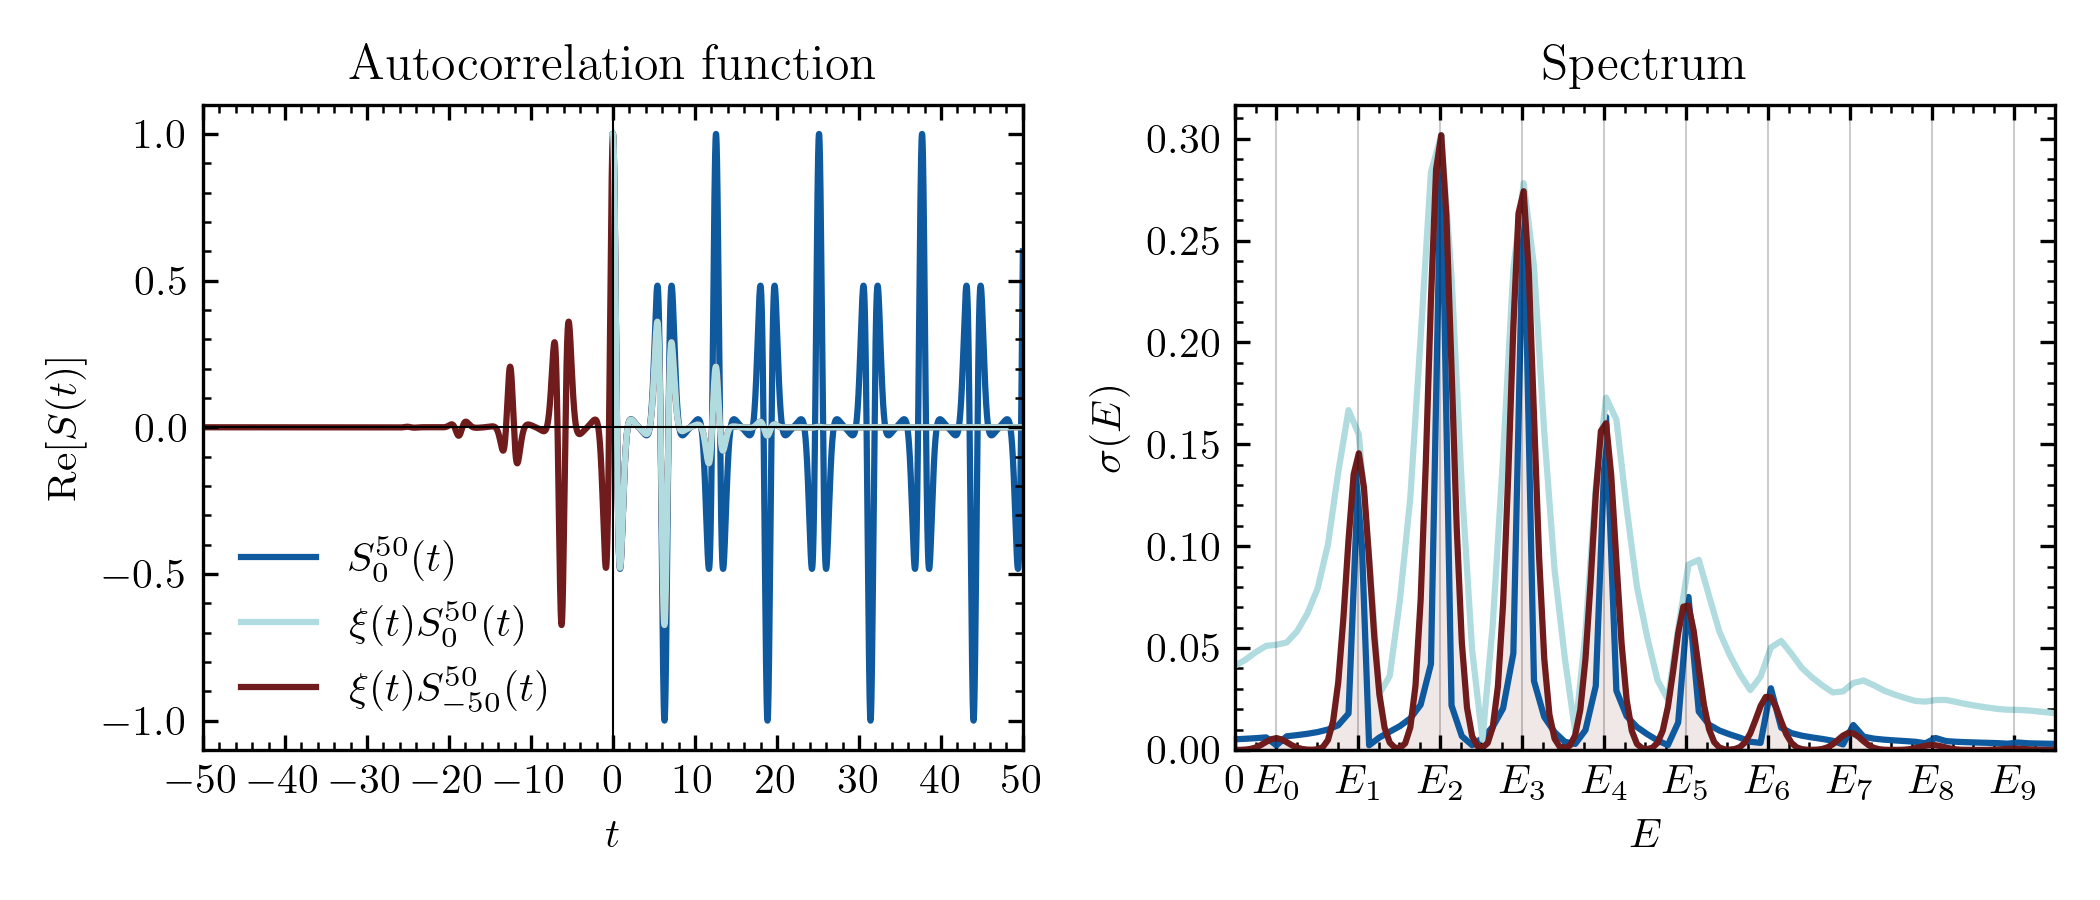
\includegraphics[width=0.9\linewidth]{scriptum/obrazky/autocorr/autocorr3.png}
    \caption{The effect of discrete \acrshort{ift} on the spectrum for undamped autocorrelation function in the range $t\in[0,50]$ ($S_0^{50}$) as obtained from the simulation, damped autocorrelation function in the range $t\in[0,50]$ ($\xi S_0^{50}$) and damped autocorrelation function spanning from -50 to 50 ($\xi S_{-50}^{50}$). While for the undamped $S_0^{50}$ the peaks remain at the correct position, the damped $\xi S_0^{50}$ has the peak maxima shifted from the exact values. Furthermore, both $S_0^{50}$ and $S_0^{50}$ have asymmetric peak shapes caused by a sharp truncation of $S$. For both the incorrect line shape decreases the resolution of the spectrum. Notice for example the region around $E_0$. While we can clearly see a small peak for $\xi S_{-50}^{50}$, there is no peak for the original data $S_{0}^{50}$ and there is only a shoulder for $\xi S_{0}^{50}$. The energy $E_0$ would be then difficult to extract for anything but $\xi S_{-50}^{50}$.}
    \label{fig:autocorr3}
\end{figure}

Finally, we conclude with a brief comment on the resolution of discrete \acrlong{ft} and \acrlong{ift}. Discrete \acrshort{ft} takes as input data represented on a grid and creates their image in the energy domain.\footnote{Fourier transform naturally provides data in the frequency domain $\nu$, which can be converted to energy domain as $E = 2 \pi \hbar \nu$.} The energy grid has the same number of grid points as the time grid, but the spacing between energy points is inversely proportional to the total time duration of the grid:
\begin{equation}
    \Delta E \propto \frac{\hbar}{t_\mathrm{max}}
\end{equation}
Thus, if we want the spectrum with higher resolution (smaller $\Delta E$), we need to extend our simulation time $t_\mathrm{max}$. Conversely, the length of the energy grid is inversely proportional to the spacing of the time grid $\Delta t$, so a finer simulation time step will extend the energy range of the spectrum. In summary, achieving a higher energy resolution (smaller $\Delta E$) requires extending the total time of the simulation, while widening the energy range requires a finer time step $\Delta t$.

\section{Code}

The essential part of calculating the autocorrelation function is again the wave function propagation, for which we have already created a code in Chapter~\ref{kap:qd}. We will reuse the code in this Chapter and modify it to calculate the spectrum from the autocorrelation function. Thus, we will only comment on the additions to the code in the following text, giving more freedom with the implementation to the reader. Still, the reader can find the full exercise code written at our \href{https://github.com/PHOTOX/QM-hands-on/blob/main/codes/exercises/autocorr.py}{Github} page.

First, we need to store the initial wave function to a separate variable and create empty lists for the autocorrelation function and time, where we will append the current values during the propagation. These additions must come in the initialization part of the code prior to the main propagation loop.
\begin{lstlisting}[language=Python, style=mystyle2]
...
# save the initial wave function for calculating the autocorrelation function
psi0 = psi  # initial wave function
time, autocorr = [], []  # empty lists for appending values of time and autocorrelation function
...
\end{lstlisting}

Then, we need to calculate the values of the autocorrelation function during the propagation (i.e., in the \python{while} loop) and store them in our array. The value of the autocorrelation function is the overlap between \python{psi} and \python{psi0,} calculated with e.g. the trapezoid rule.
\begin{lstlisting}[language=Python, style=mystyle2]
while t < simtime:  # loop until simulation time is reached
    ... # wave function propagation
    # calculate the autocorrelation function S(t) = <psi(0)|psi(t)>
    overlap =  # calculate the overlap

    autocorr.append(overlap)  # appending the overlap to our autocorrelation function list
    time.append(t)  # appending t to our time list
    ... # calculation of energies and plotting
\end{lstlisting}

These two code snippets are the only modifications of the quantum dynamics code. Once the quantum dynamics is finished, we should have the autocorrelation function calculated. Note that the most time-consuming part of the quantum dynamics code is the wave function plotting. We recommend removing the plotting functions, which will significantly speed up the code, since we focus only on the autocorrelation function after the dynamics.

Now, we need to process the autocorrelation function and calculate the energy spectrum. Since we have the data stored as lists, we convert \python{autocorr} and \python{time} into NumPy arrays first. Then, we apply the damping function \eqref{eq:damping1} and extend $S(t)$ to negative times using \eqref{eq:autocorrsym1}, both described in Section~\ref{sec:autocorr_numap}. Note that these operations can be interchanges. Finally, we used the discrete \acrshort{ift} on $S(t)$ and calculated the spectrum. All these operations are one or two-line procedures. The major part of the code is the prepared plotting of the results.
\begin{lstlisting}[language=Python, style=mystyle2]
### autocorrelation function section ###
autocorr = np.array(autocorr)  # converting the autocorrelation function to a numpy array
time = np.array(time)  # converting the time to a numpy array

# apply the damping to the autocorrelation function in form of exp(-kappa*time)
autocorr =  # apply the damping factor

# extend the autocorrelation function to negative times assuming that S(t) = S^*(-t)
time = np.concatenate([-time[::-1], time])  # new time array in range [-t_max, t_max]
autocorr = np.concatenate([np.conjugate(autocorr[::-1]), autocorr])  # new symmetric autocorr in range [-t_max, t_max]

# calculate spectrum from autocorrelation function and the frequency axis corresponding to it
spectrum = # fill in the inverse Fourier transform
freq = 2*np.pi*np.fft.fftfreq(len(time), d=dt)

# plot results
fig, axs = plt.subplots(1, 2, figsize=(8, 3), tight_layout=True)

# autocorrelation function
axs[0].plot(time, np.real(autocorr), label=r'$\mathcal{Re}[S(t)]$')
axs[0].plot(time, np.imag(autocorr), label=r'$\mathcal{Im}[S(t)]$')
axs[0].set_xlabel('Time (a.u.)')
axs[0].set_ylabel(r'$S(t)$')
axs[0].set_title('Autocorrelation Function')
axs[0].legend(frameon=False, labelspacing=0)

# spectrum
axs[1].plot(hbar*freq, np.abs(spectrum))
axs[1].set_xlim(0, np.max(hbar*freq[spectrum > np.max(spectrum)/1000]))
axs[1].set_ylim(0)
axs[1].set_xlabel('Energy (a.u.)')
axs[1].set_ylabel(r'$\mathcal{F}^{-1}[S(t)]$')
axs[1].set_title('Spectrum')

# searching for local maxima of the spectrum
print(f"\nMaxima of the spectrum:")
abs_spectrum = np.abs(spectrum)
loc_max_bool = (abs_spectrum[1:-1] > abs_spectrum[:-2]) & (abs_spectrum[1:-1] > abs_spectrum[2:])
loc_max_index = np.where(loc_max_bool)[0] + 1
loc_max_energies = hbar*freq[loc_max_index]
for index, en in enumerate(loc_max_energies):
    intensity = abs_spectrum[loc_max_index[index]]
    print(f" * State {index}: E = {en:.5f} a.u.; I = {intensity:.5e}")
    axs[1].axvline(en, lw=1, color='black', alpha=0.1)
    axs[1].scatter(en, intensity, marker='x', color='black', s=20)

plt.show()
\end{lstlisting}

\section{Applications}

\subsection*{Exercise: Energy spectrum of a harmonic oscillator}

The spectrum of a harmonic oscillator (Eq.~\eqref{eq:qdho}) is derived in all introductory courses to quantum mechanics and takes a very simple form:
\begin{equation*}
    E_n^\mathrm{HO} = \hbar\omega\left(n+\frac{1}{2}\right) \quad n=0,1,2,\dots \, .
\end{equation*}
The derivation of the spectrum is a typical example of the Hamiltonian diagonalization, which is the time-independent approach. In this exercise, we will contrast the exact spectrum with the spectrum calculated by the time-dependent approach presented in this Chapter.

\paragraph{Assignment:} Set up a harmonic oscillator from Eq.~\eqref{eq:qdho} and an initial Gaussian wave packet from Eq~\eqref{eq:qdgauss} with the following parameters: $m=1$~a.u., $\omega=0.1$~a.u., $x_0=6$~a.u., $p_0=0$~a.u. and $\alpha_0 = 0.3$. Propagate the wave packet for at least 10000~a.u. Don't forget to set a corresponding grid and time step! Then, apply the Gaussian damping function \eqref{eq:gaussdamping} with the parameter $\gamma = 0.005$. Do the peak positions correspond to the energies of the harmonic oscillator $E_n^\mathrm{HO}$? Try also values of $\gamma=0.02$, 0.05 and 0.1. Can you still distinguish all the peaks in the spectrum? Try to find the limit of $\gamma$ where the peaks can be still distinguished and energies clearly estimated.

\subsection*{Exercise: Initial wave function effect on the spectrum}

The spectrum calculated from the autocorrelation function depends on the initial wave function, namely on the magnitude of the expansion coefficients $c_k$. Thus, if $c_k = 0$ for some state, there will be no peak at $E_k$ in the spectrum and we will be blind to this eigenvalue of the Hamiltonian. Since the spectrum depends on the initial wave function through its expansion coefficients $c_k$, the number and intensity of peaks can be modified by changing the initial wave function for the dynamics. In this exercise, we will explore the effect of the initial wave function on the spectrum. 

\paragraph{Assignment:} Use the potential from the previous Exercise with the damping parameter $\gamma = 0.005$. Start with the Gaussian function with $x_0=0$~a.u., $p_0=0$~a.u. and $\alpha_0 = 0.5$, and examine the spectrum. Do you see the full spectrum of the harmonic oscillator? Test what happens if $x_0=0.1$ and 0.5~a.u. Can you explain your observation? Hint: think about the symmetry of the potential an the initial guess. Finally, try to optimize the initial wave function to obtain a maximum number of clearly identifiable peaks in the spectrum. Note that you can change also the initial wave function form.

% \subsection*{*Exercise: Degeneracies in the spectrum}

% Use double-well potential..

% \paragraph{Assignment:} 


% \subsection*{*Exercise: Spectrum of Auger decay}

% \paragraph{Assignment:} 


%%%%%%%%%%%%%%%%%%%%%%%%%%%%%%%%%%%%%%%%%%%%%%%%%%%
%%%%%%%%%%%%%% Don't remove!!! %%%%%%%%%%%%%%%%%%%%
%%%%%%%%%%%%%%%%%%%%%%%%%%%%%%%%%%%%%%%%%%%%%%%%%%%

% \section{*Connection to spectroscopy}

% We will close this Chapter with some remarks on computational spectroscopy. The reader have probably heard about the first-order perturbation theory which allow to derive the Fermi's golden rule. The formula for absorption spectrum in terms of 
% \begin{equation*}
%     \sigma (\omega) = \frac{4\pi^2\omega}{3 c \hbar} \sum_{\nu} |\langle \psi_{f\nu'} | \Vec{\mu} | \psi_{i\nu} \rangle |^2 \delta(\omega - \Delta \omega) \, ,
% \end{equation*}
% where $c$ is the speed of light, $\psi_{i\nu}$ is the initial wave function in $i$-th electronic and $\nu$-th vibrational state, $\psi_{f\nu'}$ is the final wave function in $f$-th electronic and $\nu'$-th vibrational state and $\Delta \omega$ is frequency difference between the initial and final states:
% \begin{equation*}
%     \Delta \omega = \frac{E_{f\nu'}-E_{i\nu}}{\hbar} \, .
% \end{equation*}
% This formula, well known to students of theoretical chemistry, can be reformulated as
% \begin{equation*}
%     \sigma (\omega) = \frac{2\pi\omega}{3 c \hbar} \int_{-\infty}^\infty \langle \psi_{i\nu} | \Vec{\mu}^* \e^{-i\hat{H}_ft/\hbar} \Vec{\mu} \e^{i\hat{H}_i t/\hbar} | \psi_{i\nu} \rangle \dd t \, .
% \end{equation*}